\documentclass{article}

% if you need to pass options to natbib, use, e.g.:
%     \PassOptionsToPackage{numbers, compress}{natbib}
% before loading neurips_2018

% ready for submission
% \usepackage{neurips_2018}

% to compile a preprint version, e.g., for submission to arXiv, add add the
% [preprint] option:
%     \usepackage[preprint]{neurips_2018}

% to compile a camera-ready version, add the [final] option, e.g.:
% \usepackage[final]{neurips_2018}

% to avoid loading the natbib package, add option nonatbib:
%     \usepackage[nonatbib]{neurips_2018}

\usepackage[utf8]{inputenc} % allow utf-8 input
\usepackage[T1]{fontenc}    % use 8-bit T1 fonts
\usepackage{hyperref}       % hyperlinks
\usepackage{url}            % simple URL typesetting
\usepackage{booktabs}       % professional-quality tables
\usepackage{amsfonts}       % blackboard math symbols
\usepackage{nicefrac}       % compact symbols for 1/2, etc.
\usepackage{microtype}      % microtypography

\usepackage{amsmath,amsthm,amssymb}
\usepackage{mathtools}
\DeclareMathOperator*{\argmin}{argmin}
\DeclareMathOperator*{\argmax}{argmax}
\usepackage{graphicx}
\graphicspath{{./images/}}
\usepackage{float}

\title{Empirical Assessment of HMM and HSMM Accuracy}

% The \author macro works with any number of authors. There are two commands
% used to separate the names and addresses of multiple authors: \And and \AND.
%
% Using \And between authors leaves it to LaTeX to determine where to break the
% lines. Using \AND forces a line break at that point. So, if LaTeX puts 3 of 4
% authors names on the first line, and the last on the second line, try using
% \AND instead of \And before the third author name.

\author{%
  Albert Lam, Kabir Sawhney, and Joey Yoo \\
  \texttt{albertlam, ksawhney, joeyyoo@uchicago.edu} \\
  % examples of more authors
  % \And
  % Coauthor \\
  % Affiliation \\
  % Address \\
  % \texttt{email} \\
  % \AND
  % Coauthor \\
  % Affiliation \\
  % Address \\
  % \texttt{email} \\
  % \And
  % Coauthor \\
  % Affiliation \\
  % Address \\
  % \texttt{email} \\
  % \And
  % Coauthor \\
  % Affiliation \\
  % Address \\
  % \texttt{email} \\
}

\begin{document}
% \nipsfinalcopy is no longer used

\maketitle

\begin{abstract}
We empirically compare the accuracy of the Baum-Welch and Viterbi algorithms with a Hidden Semi-Markov Model (HSMM) algorithm to estimate hidden state sequences from time-ordered observations. Specifically, we simulate agent pathways in a variety of GridWorld settings that differ in grid size, placement of obstacles, and transition mechanism, including settings which violate the Markov assumption implicit to a Hidden Markov Model (HMM). We found that (to be filled in)
\end{abstract}

\section{Background and Introduction}

Algorithms to estimate the most likely sequence of hidden states from observations in a hidden Markov model rely on the Markov assumption, that future states are conditionally independent of past states given the present state. The most popular method for estimating these states involves evaluating conditional likelihood using the forward-backward algorithm and then inferring the most likely sequence of hidden states using the Viterbi algorithm, which relies on this assumption. However, some researchers have suggested that the Markov assumption need not be strictly met for these techniques to generate reasonably accurate estimates of hidden state sequences. We sought to empirically test this proposition on the problem of estimating an agent's path in a GridWorld setting. To do so, we randomly generated a sequence of robot movements and observations under a variety of assumptions, including settings where we enforced the Markov assumption and others where we relaxed it.

\subsection{Hidden Markov Model (HMM)}
A HMM is a model consisting of two sequences:
\begin{itemize}
  \item A state sequence $z = \{z_1, z_2, \dots, z_T\}$ where $z_t$ is the state at timestep $t$ which takes a value from a state space $\mathcal{Z}$ that is assumed to be static and finite for $t = 1, 2, \dots, T$.
  \item An observation (or emission) sequence $x = \{x_1, x_2, \dots, x_T\}$ where $x_t$ is the observation at timestep $t$ from an observation space $\mathcal{X}$ that is assumed to be static and finite for $t = 1, 2, \dots, T$.
\end{itemize}

The relationship between these two sequences are embedded in the transition probabilities and the emission probabilities of the HMM. In particular, let $\pi_{i,j} = \mathbb{P}(z_{t+1} = j | z_{t} = i)$ denote the probability of an agent transitioning from state $i$ to state $j$, which we assume to be independent of $t$, and $\mathbb{P}(z_t = \zeta | x_t = \xi)$ denote the probability of observing $\zeta$ given state $\xi$. Interpreting these probabilities as parameters of the HMM gives way to a natural parametric Bayesian approach to estimating these probabilities that involves augmenting and then marginalizing the joint distributions of $x$ and $z$, solving for forward and backward recursions, and then computing the maximum likelihood estimates via the Baum Welch algorithm. The transition and emission probabilities can finally be used to compute most-likely trajectories using the Viterbi algorithm.

\subsection{Hidden Semi-Markov Model (HSMM)}
A HSMM extends a HMM to settings where the sequence of states are not strictly Markovian - instead, the probability of transitioning to a new state $z_{s+1}$ depends on the elapsed time in the current state $z_s$. Here, we introduce $s = 1, \dots, S$ to index state transitions that remain Markovian, and use $t= 1, \dots, T$ to index the associated emissions that are not necessarily Markovian. Then, let $D_s \in [1, \dots, T]$ denote the duration that an agent remains in state $x_s$ with explicit mass function $\mathbb{P}(D_s = d_s | z_s = i)$. Figure ~\ref{fig:hsmm} illustrates such an explicit-duration HSMM, where we define $z_s$ as super-states of sub-states $z'_{t}$ which each emit one observation $x_{t}$. It follows that the super-states are Markovian but sub-states are not.

\begin{figure}[H]
\centering
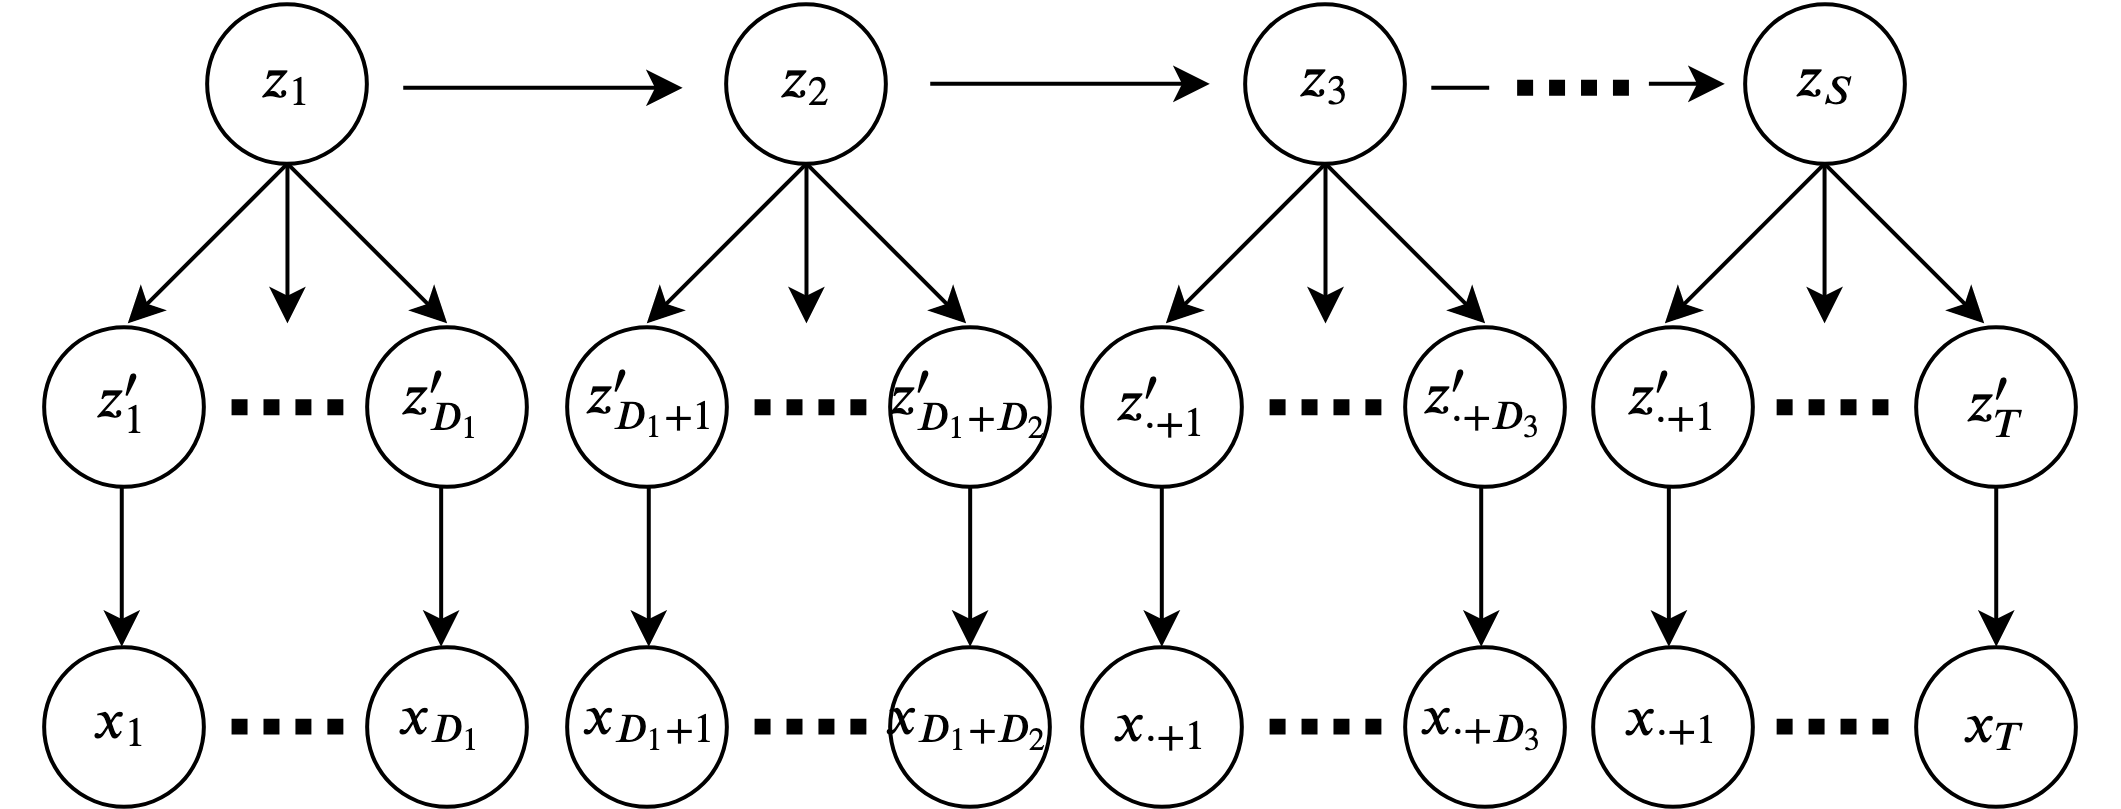
\includegraphics[scale=0.15]{images/hsmm2.png}
\caption{HSMM where super state transitions are Markovian, while emissions associated with each state follow some explicit duration distribution.}
\label{fig:hsmm}
\end{figure}

\subsection{Hierarchical Dirichlet Process HSMM (HDP-HSMM)}
We begin this section by reviewing the formulation of a hierarchical Dirichlet process HMM (HDP-HMM), which is a Bayesian non-parametric treatment of the classical HMM. A HDP-HMM$(\gamma, \alpha, H)$ model is a process governed by:
\begin{itemize}
  \item $\beta_k \coloneqq \beta_k'\cdot \prod_{i=1}^{k-1} (1-\beta_i')$ where $\beta_i' \overset{\text{i.i.d}}{\sim} Beta(1,\gamma)$
  \item $\pi_k \overset{\text{i.i.d}}{\sim} DP(H(\beta), \alpha)$ for $k = 1, \dots, \infty$ where $\beta = \{\beta_k\}_{k=1}^{\infty}$
  \item $z_t \sim \pi_{z_{t-1}}$
  \item $x_t \sim h(\theta_{z_t})$ where $\theta_{k} \sim H$ for $k = 1, \dots, \infty$
\end{itemize}
where $\gamma, \alpha > 0$ can be interpreted as concentration parameters and $H$ is the base distribution of the Dirichlet process. Note that $\{\beta_k\}_{k=1}^{\infty}$ is generated from a stick-breaking process with concentration parameter $\gamma$. These are then used in the generation of  transition distributions $\{\pi_k \}_{k=1}^{\infty}$ from a Dirichlet process with parameters $H$ and $\alpha$, where $H$ is defined on the $\{\beta_k\}_{k=1}^{\infty}$ partitions of the measurement set. For $t = 1, \dots, T$, each state $z_t$ is drawn from a respective $\pi_{z_{t-1}}$, and each observation is drawn from an observation distribution $h(\theta_{z_t})$ where $\theta_{k}$ is drawn from $H$. Observe that as $\alpha$ decreases, distributions $\{\pi_k\}_{s=1}^{\infty}$ tend to be more concentrated, and as $\gamma$ decreases, $\{\beta_k\}_{k=1}^{\infty}$ tends to zero and $\{h(\theta_{z_t})\}_{t=1}^{T}$ tends to be more concentrated as a result.

HDP-HSMM is an augmentation of the HDP-HMM to include duration distributions. Continuing from the notation above yields:
\begin{itemize}
  \item $\beta_k \coloneqq \beta_k'\cdot \prod_{i=1}^{k-1} (1-\beta_i')$ where $\beta_i' \overset{\text{i.i.d}}{\sim} Beta(1,\gamma)$
  \item $\pi_k \overset{\text{i.i.d}}{\sim} DP(H(\beta), \alpha)$ for $k = 1, \dots, \infty$ where $\beta = \{\beta_k\}_{k=1}^{\infty}$
  \item $z_s \sim \tilde{\pi}_{z_{s-1}}$
  \item $D_s \sim g(\omega_{z_s})$ where $\omega_k \sim G$ for $k = 1, \dots, \infty$
  \item $z'_{t_{s}:t'_{s}} = z_s$ where $t_{s} = \sum_{s' < s} D_s + 1$ and $t'_{s} = t_{s} + D_s - 1$
  \item $x_{t_{s}: t'_{s}} \overset{\text{i.i.d}}{\sim} h(\theta_{z'_t})$ where $\theta_{k} \sim H$ for $k = 1, \dots, \infty$
\end{itemize}

The main differences here are that we introduce a base distribution $G$ for drawing durations $D_s$ in a similar way that $H$ is defined in the HSMM setting which we use for drawing $\pi$. The duration distribution sequence of sub-states $z'_{t_{s}:t'_{s}}$ is set to the corresponding super-state $z_{s}$ where $t_{s}$ is the starting index for the sub-state sequence corresponding to super-state $z_s$, and $t'_{s}$ is the end index for the sub-state sequence corresponding to super-state $z_s$. The observation sequence is then drawn from the sub-state sequence using $H$. Note that $z_s$ is drawn from $\tilde{pi}_{k} \coloneqq \frac{\pi_{k,j}}{1-\pi_{k,k}}(1 - \delta_{k,j})$, which normalizes $\pi_k$ to prevent self-transitions in the super-state sequence $z_s$. Figure ~\ref{fig:hdphsmm} extends the previous HSMM diagram to illustrate the connections between the HDP component of the model, and the HSMM.

\begin{figure}[H]
\centering
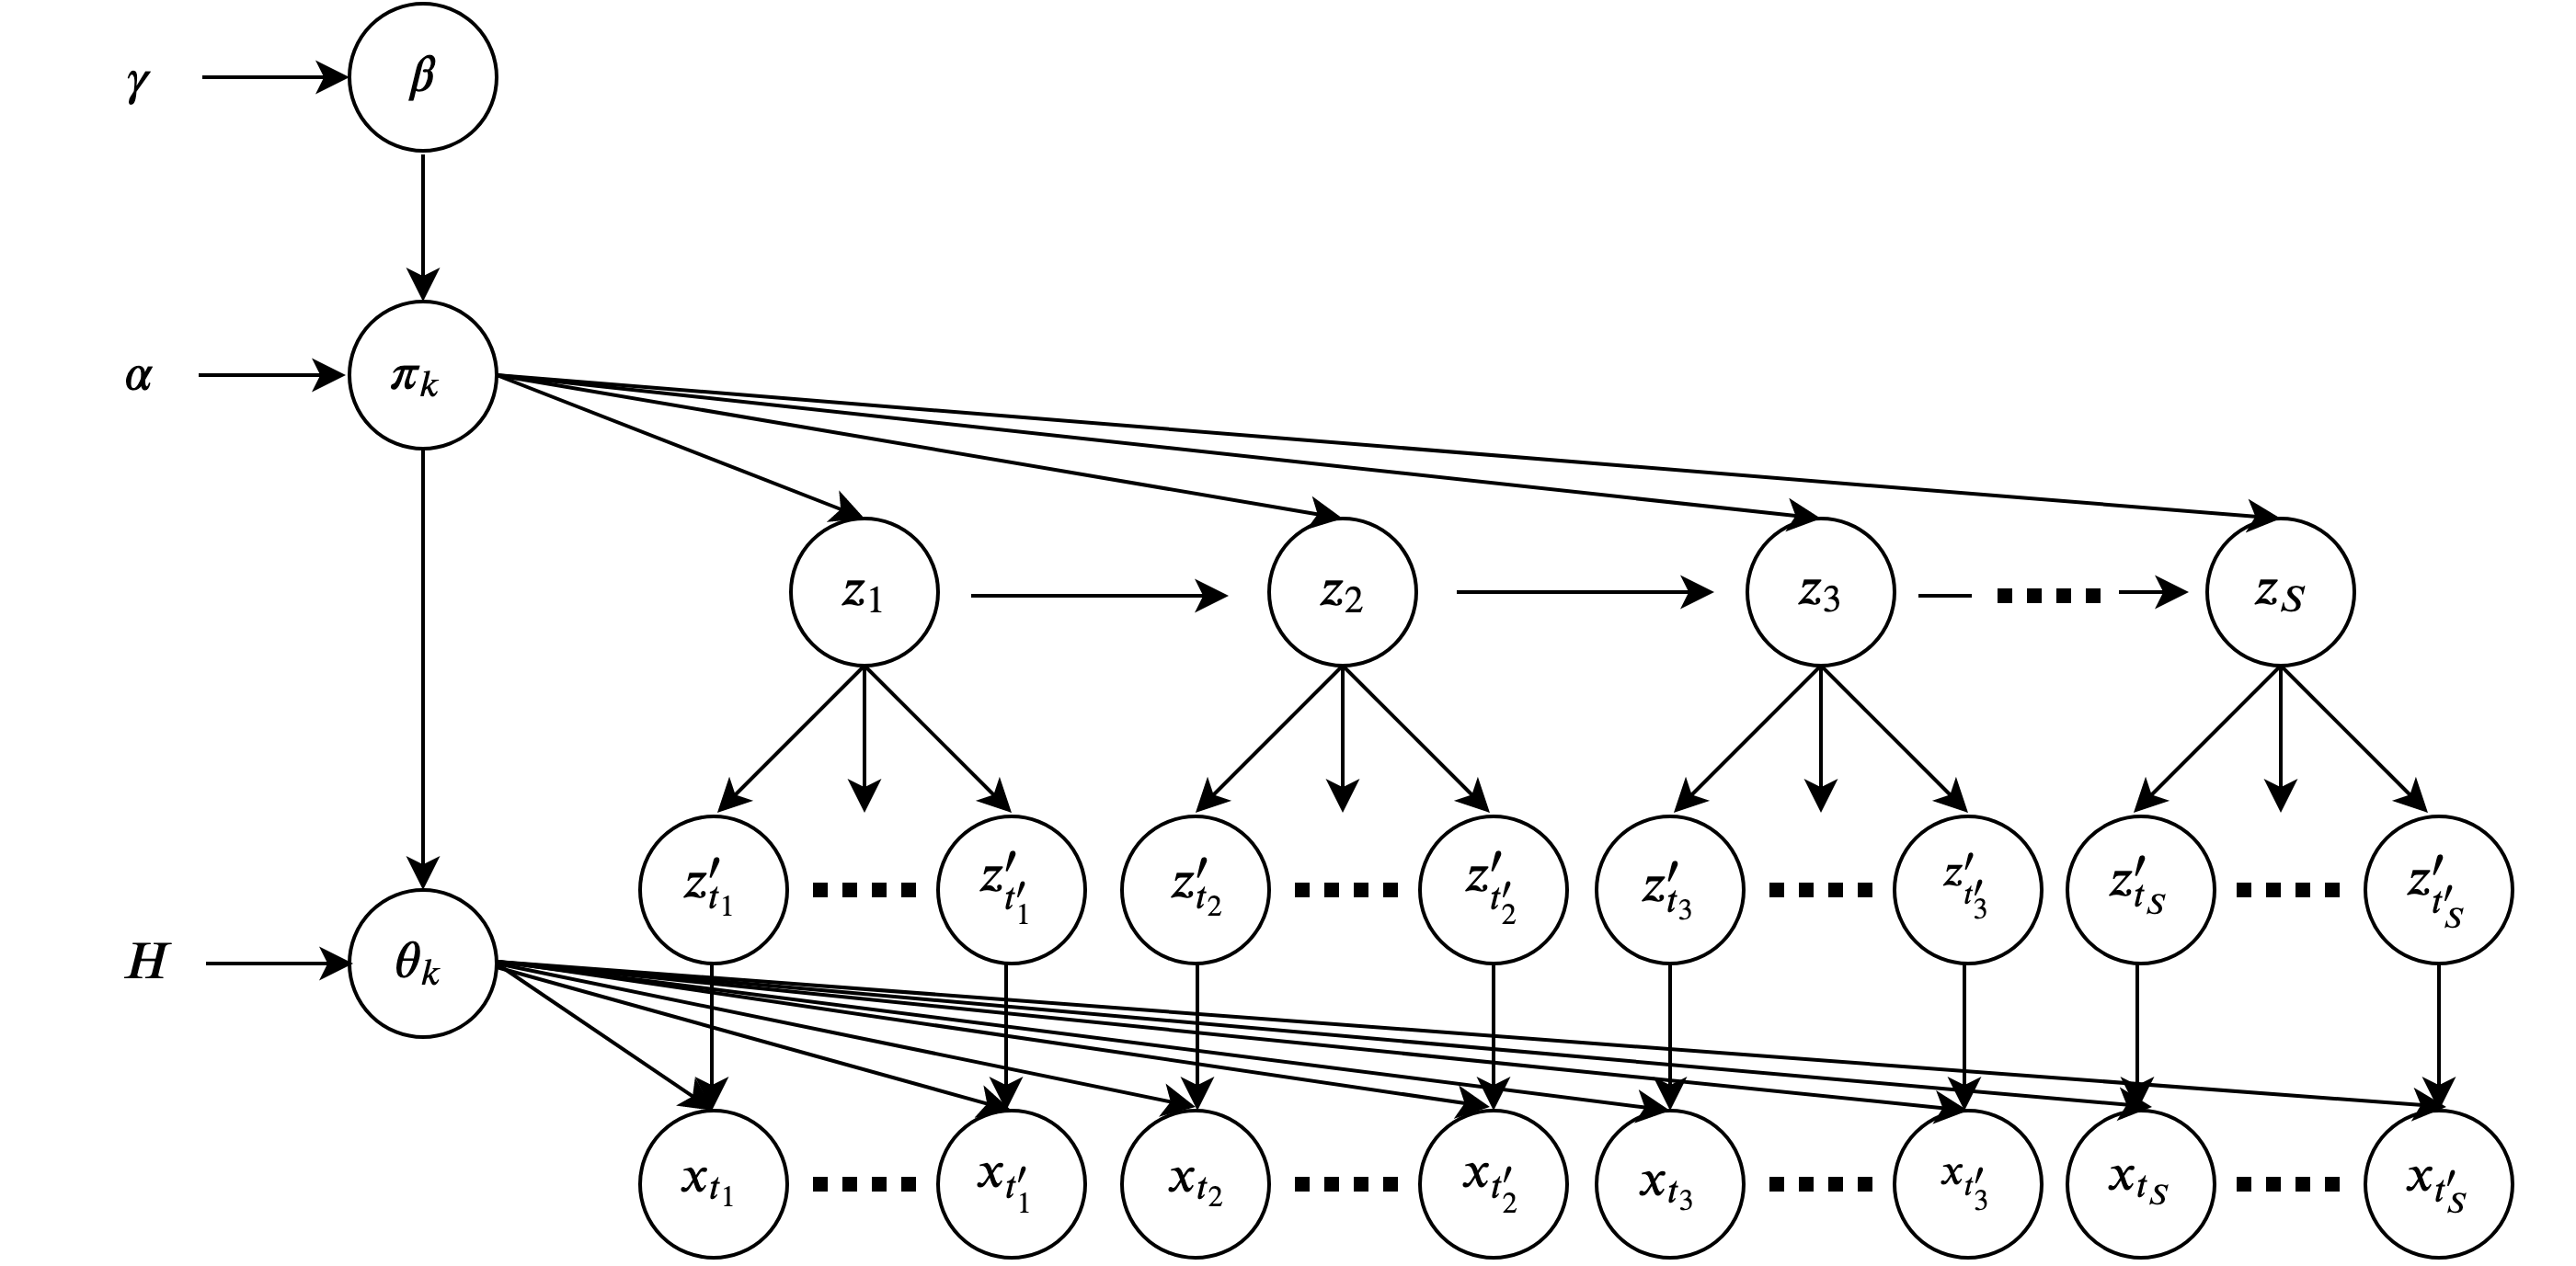
\includegraphics[scale=0.12]{images/hdphsmm.png}
\caption{HDP-HSMM incorporates a HDP component into a HSMM}
\label{fig:hdphsmm}
\end{figure}

\section{Simulating Robot States and Observations}

To generate the simulated agent pathways and observations, we varied the following map settings and motion model assumptions:

\begin{enumerate}
	\item \textbf{Map size}: We generated pathways on 5$\times$5 grids, so each grid has 25 hidden states.
	\item \textbf{Obstacles}: For each map, we placed obstacles in the map by making certain states in the grid impossible to visit -- this represents the robot encountering real-life obstacles, like walls or other objects. We varied the number and placement of obstacles in each map. We believe that increasing the number of obstacles will increase the accuracy of the estimation methods, as there are fewer possible paths for the robot to take.
	\item \textbf{Markov property}: We simulated three different settings for the transition matrix between states, two of which did not violate the Markov assumption and one that did. Further details of these settings are Section 2.2 below.
\end{enumerate}

\subsection{GridWorld Setup}

We simulated the robot pathways on the following three grids. Each square in the grid either has a number representing its true observation, or is colored black, indicating an obstacle.

\newcommand{\addmapa}{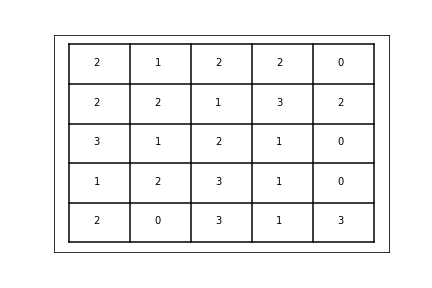
\includegraphics[width=10em]{data/Profile_1/mapping.png}}
\newcommand{\addmapb}{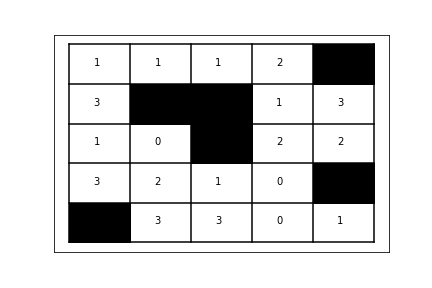
\includegraphics[width=10em]{data/Profile_2/mapping.png}}
\newcommand{\addmapc}{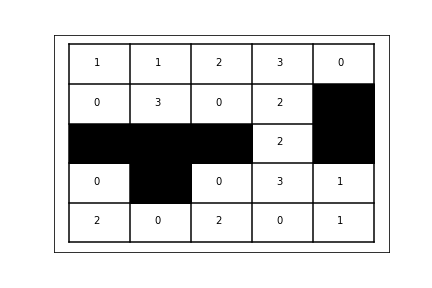
\includegraphics[width=10em]{data/Profile_3/mapping.png}}
\newcolumntype{C}{>{\centering\arraybackslash}m{10em}}
\begin{table}[H]
\sffamily
\centering
\begin{tabular}{l*4{C}@{}}
& \addmapa & \addmapb & \addmapc \\
\end{tabular}
\caption{Gridworld models}
\end{table} 


\subsection{Robot Motion Settings}

As stated above, the robot path for each grid was simulated using three different settings for the transitions between states.

\begin{enumerate}
	\item \textbf{Purely random}: The robot randomly transitions from state to state, with a uniform transition probability over all of the states (including its current state). Therefore, the state sequence is essentially purely random, with each step randomly generated with replacement from the set of available states. This setting satisfies the Markov property, as each time step is independent from all other time steps.
	\item \textbf{Traditional Markov}: The state sequences are generated using a fixed transition matrix -- the probability of transitioning from one state to the next is constant as the sequence is generated (with one state selected as the starting state), and each step is independent of past states conditional on the present state. This setting satisfies the Markov property, so we would expect the HMM method to do well on the data simulated from it, in both estimating the transition probability matrix and in the accuracy of the maximum likelihood state sequence.
	\item \textbf{Changing transition matrix (Stickiness}: HSMM specializes in inferring the observations when the transition is sticky. Sticky property is where the transition probability changes relative to how long the robot stays in the same state. The transition probability of staying in the same state decreases linearly by the number of time the robot is in the same state. If the robot moves to a different state, the transition matrix returns to the original one that we started from.
 \end{enumerate}

\subsection{Robot Observation Settings}

To compare the original HMM and HSMM together, we have modified the observation to be continuous. Each state is distinguished by its distinct mean, while the sigma is initialized to be the same across all state. The mean value is similar to the discrete setting, the value of 0, 1, 2, or 3. In each state, the robot observes a normal sample given the mu of the state.

To generate our data, for each of the 9 settings (3 grids x 3 transition settings), we simulated 200 state sequences of varying lengths. Then, we simulated observations from these state sequences using the randomly generated emission matrices (the "true" observation for each state was also randomly assigned). These generated observation sequences then became the input for our HMM and HSMM algorithms.


\section{Headings: first level}
\label{headings}

All headings should be lower case (except for first word and proper nouns),
flush left, and bold.

First-level headings should be in 12-point type.

\subsection{Headings: second level}

Second-level headings should be in 10-point type.

\subsubsection{Headings: third level}

Third-level headings should be in 10-point type.

\paragraph{Paragraphs}

There is also a \verb+\paragraph+ command available, which sets the heading in
bold, flush left, and inline with the text, with the heading followed by 1\,em
of space.

\section{Citations, figures, tables, references}
\label{others}

These instructions apply to everyone.

\subsection{Citations within the text}

The \verb+natbib+ package will be loaded for you by default.  Citations may be
author/year or numeric, as long as you maintain internal consistency.  As to the
format of the references themselves, any style is acceptable as long as it is
used consistently.

The documentation for \verb+natbib+ may be found at
\begin{center}
  \url{http://mirrors.ctan.org/macros/latex/contrib/natbib/natnotes.pdf}
\end{center}
Of note is the command \verb+\citet+, which produces citations appropriate for
use in inline text.  For example,
\begin{verbatim}
   \citet{hasselmo} investigated\dots
\end{verbatim}
produces
\begin{quote}
  Hasselmo, et al.\ (1995) investigated\dots
\end{quote}

If you wish to load the \verb+natbib+ package with options, you may add the
following before loading the \verb+neurips_2018+ package:
\begin{verbatim}
   \PassOptionsToPackage{options}{natbib}
\end{verbatim}

If \verb+natbib+ clashes with another package you load, you can add the optional
argument \verb+nonatbib+ when loading the style file:
\begin{verbatim}
   \usepackage[nonatbib]{neurips_2018}
\end{verbatim}

As submission is double blind, refer to your own published work in the third
person. That is, use ``In the previous work of Jones et al.\ [4],'' not ``In our
previous work [4].'' If you cite your other papers that are not widely available
(e.g., a journal paper under review), use anonymous author names in the
citation, e.g., an author of the form ``A.\ Anonymous.''

\subsection{Footnotes}

Footnotes should be used sparingly.  If you do require a footnote, indicate
footnotes with a number\footnote{Sample of the first footnote.} in the
text. Place the footnotes at the bottom of the page on which they appear.
Precede the footnote with a horizontal rule of 2~inches (12~picas).

Note that footnotes are properly typeset \emph{after} punctuation
marks.\footnote{As in this example.}

\subsection{Figures}

\begin{figure}
  \centering
  \fbox{\rule[-.5cm]{0cm}{4cm} \rule[-.5cm]{4cm}{0cm}}
  \caption{Sample figure caption.}
\end{figure}

All artwork must be neat, clean, and legible. Lines should be dark enough for
purposes of reproduction. The figure number and caption always appear after the
figure. Place one line space before the figure caption and one line space after
the figure. The figure caption should be lower case (except for first word and
proper nouns); figures are numbered consecutively.

You may use color figures.  However, it is best for the figure captions and the
paper body to be legible if the paper is printed in either black/white or in
color.

\subsection{Tables}

All tables must be centered, neat, clean and legible.  The table number and
title always appear before the table.  See Table~\ref{sample-table}.

Place one line space before the table title, one line space after the
table title, and one line space after the table. The table title must
be lower case (except for first word and proper nouns); tables are
numbered consecutively.

Note that publication-quality tables \emph{do not contain vertical rules.} We
strongly suggest the use of the \verb+booktabs+ package, which allows for
typesetting high-quality, professional tables:
\begin{center}
  \url{https://www.ctan.org/pkg/booktabs}
\end{center}
This package was used to typeset Table~\ref{sample-table}.

\begin{table}
  \caption{Sample table title}
  \label{sample-table}
  \centering
  \begin{tabular}{lll}
    \toprule
    \multicolumn{2}{c}{Part}                   \\
    \cmidrule(r){1-2}
    Name     & Description     & Size ($\mu$m) \\
    \midrule
    Dendrite & Input terminal  & $\sim$100     \\
    Axon     & Output terminal & $\sim$10      \\
    Soma     & Cell body       & up to $10^6$  \\
    \bottomrule
  \end{tabular}
\end{table}

\section{Final instructions}

Do not change any aspects of the formatting parameters in the style files.  In
particular, do not modify the width or length of the rectangle the text should
fit into, and do not change font sizes (except perhaps in the
\textbf{References} section; see below). Please note that pages should be
numbered.

\section{Preparing PDF files}

Please prepare submission files with paper size ``US Letter,'' and not, for
example, ``A4.''

Fonts were the main cause of problems in the past years. Your PDF file must only
contain Type 1 or Embedded TrueType fonts. Here are a few instructions to
achieve this.

\begin{itemize}

\item You should directly generate PDF files using \verb+pdflatex+.

\item You can check which fonts a PDF files uses.  In Acrobat Reader, select the
  menu Files$>$Document Properties$>$Fonts and select Show All Fonts. You can
  also use the program \verb+pdffonts+ which comes with \verb+xpdf+ and is
  available out-of-the-box on most Linux machines.

\item The IEEE has recommendations for generating PDF files whose fonts are also
  acceptable for NeurIPS. Please see
  \url{http://www.emfield.org/icuwb2010/downloads/IEEE-PDF-SpecV32.pdf}

\item \verb+xfig+ "patterned" shapes are implemented with bitmap fonts.  Use
  "solid" shapes instead.

\item The \verb+\bbold+ package almost always uses bitmap fonts.  You should use
  the equivalent AMS Fonts:
\begin{verbatim}
   \usepackage{amsfonts}
\end{verbatim}
followed by, e.g., \verb+\mathbb{R}+, \verb+\mathbb{N}+, or \verb+\mathbb{C}+
for $\mathbb{R}$, $\mathbb{N}$ or $\mathbb{C}$.  You can also use the following
workaround for reals, natural and complex:
\begin{verbatim}
   \newcommand{\RR}{I\!\!R} %real numbers
   \newcommand{\Nat}{I\!\!N} %natural numbers
   \newcommand{\CC}{I\!\!\!\!C} %complex numbers
\end{verbatim}
Note that \verb+amsfonts+ is automatically loaded by the \verb+amssymb+ package.

\end{itemize}

If your file contains type 3 fonts or non embedded TrueType fonts, we will ask
you to fix it.

\subsection{Margins in \LaTeX{}}

Most of the margin problems come from figures positioned by hand using
\verb+\special+ or other commands. We suggest using the command
\verb+\includegraphics+ from the \verb+graphicx+ package. Always specify the
figure width as a multiple of the line width as in the example below:
\begin{verbatim}
   \usepackage[pdftex]{graphicx} ...
   \includegraphics[width=0.8\linewidth]{myfile.pdf}
\end{verbatim}
See Section 4.4 in the graphics bundle documentation
(\url{http://mirrors.ctan.org/macros/latex/required/graphics/grfguide.pdf})

A number of width problems arise when \LaTeX{} cannot properly hyphenate a
line. Please give LaTeX hyphenation hints using the \verb+\-+ command when
necessary.

\subsubsection*{Acknowledgments}

Use unnumbered third level headings for the acknowledgments. All acknowledgments
go at the end of the paper. Do not include acknowledgments in the anonymized
submission, only in the final paper.

\section*{References}

References follow the acknowledgments. Use unnumbered first-level heading for
the references. Any choice of citation style is acceptable as long as you are
consistent. It is permissible to reduce the font size to \verb+small+ (9 point)
when listing the references. {\bf Remember that you can use more than eight
  pages as long as the additional pages contain \emph{only} cited references.}
\medskip

\small

[1] Johnson, M.J.\ \& Willsky, A.S.\ (2013) Bayesian Nonparametric Hidden Semi-Markov Models, {\it Journal of Machine Learning Research 14 (2013)},
pp.\ 673--701. Cambridge, MA: MIT Press.

\end{document}